\section{The Projected Grid}
The projected grid is based on a simple concept: in order to achieve an
uniform distribution of details on the image plane, a uniformly spaced grid is
created in post-perspective space and transformed back to world space.
Figure~\ref{fig:projectedgrid} illustrates the difference between a classic
world space approach and the projected grid.
\begin{figure}[h]
\centering
\subbottom[Increase]
{
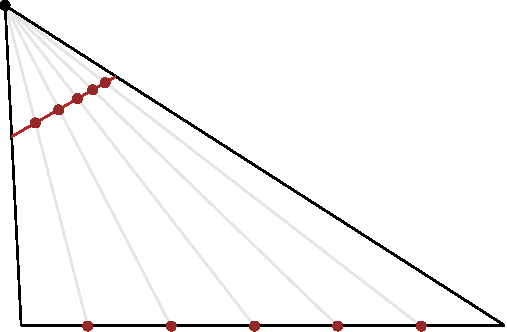
\includegraphics[scale=0.75]{figures/ProjectedGridVsWorldSpace.pdf}
\label{fig:subfigprojgrid1}
}
\subbottom[Increase]
{
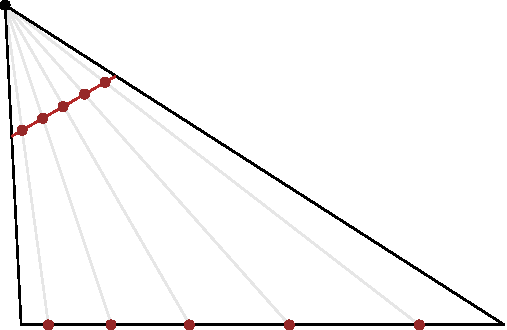
\includegraphics[scale=0.75]{figures/ProjectedGridUniform.pdf}
\label{fig:subfigprojgrid2}
}
\caption[The Projected Grid Concept]{The image on the left
~\subcaptionref{fig:subfigprojgrid1} shows an uniform grid in worldspace, it's
projection onto the image plane is not uniformly spaced though. The image on the
right~\subcaptionref{fig:subfigprojgrid2} on the other hand depicts an uniform grid on
the image plane and its associated non-uniform spaced worldspace positions.}
\label{fig:projectedgrid}
\end{figure}

% The algorithm used for the projected grid can be broken down into the following
% steps:
% \begin{itemize}
%  \item create a uniformly spaced grid orthogonal to the viewer using normalised
% device coordinates
%  \item transform the grid to worldspace
%  \item project the grid onto the desired base plane
%  \item apply height displacement
%  \item run the grid through the rendering pipeline as usual
% \end{itemize}

% Typically, vertices in world space are transformed to clip space through application
% of the combined view and projection matrix. After clipping has been performed, the
% resulting vertices are converted to normalised device coordinates by performing the
% perspective division.
% 
% 
% Clip Coordinates result from transforming Eye Coordinates by the Projection matrix.
% Clip Coordinate space ranges from -Wc to Wc in all three axes, where Wc is the Clip
% Coordinate W value. OpenGL clips all coordinates outside this range.
% 
% Perspective division performed on the Clip Coordinates produces Normalized Device
% Coordinates, ranging from -1 to 1 in all three axes.

Let $\mathbf{x}$ be a column vector representing the homogeneous world space
coordinates of a vertex, $\mathbf{V}$ the view matrix and $\mathbf{P}$ the
projection matrix, then
\begin{equation}
 \mathbf{c} = \mathbf{P} \mathbf{V} \mathbf{x}
\end{equation}
where $\mathbf{c}$ lies in clip space. The three dimensional viewing volume for
a vertex $\mathbf{c}$ in clip space is defined as
\begin{equation}
 \mathbf{c}_x, \mathbf{c}_y, \mathbf{c}_z \in \interval{-\mathbf{c}_w}{\mathbf{c}_w}
\end{equation}
In case one or more of $\mathbf{c}_x$, $\mathbf{c}_y$ and $\mathbf{c}_z$ are outside
the range defined by $\mathbf{c}_w}$, the vertex is clipped.

\begin{equation}
 \mathbf{n} = \frac{1}{\mathbf{c}_w}(\mathbf{c}_x, \mathbf{c}_y, \mathbf{c}_z)^\mathsf{T}
\end{equation}

The clip space vertices are calculated like the following:
Homogenise clip space coordinates, the result are normalised device coordinates.


The projected grid on the other hand starts inside the canonical view volume,
and needs to transform the vertices back to world space. The matrix used
herefore may look like the following:
\begin{align}
 \mathbf{M}_{inv}& = (\mathbf{M}_{proj} \cdot \mathbf{M}_{view})^{-1}\\
 \mathbf{x}_{hw}& = \mathbf{M}_{inv} \cdot \mathbf{x}_{clip}\\
 \mathbf{x}_{world}& = homogenize(\mathbf{x}_{hw})
\end{align}

\begin{align}
 \mathbf{x}_{near}& = \begin{pmatrix} x & y & -1 & 1 \end{pmatrix} && x,y \in \interval{-1}{1}\\
 \mathbf{x}_{far}& = \begin{pmatrix} x & y & 1 & 1 \end{pmatrix}
\end{align}

Apply the matrix to the vertices:
\begin{equation}
 \mathbf{x_{w}} = \mathbf{M_{inv}} \cdot \mathbf{x_{c}}
\end{equation}

Homogenise the coordinates:
\begin{equation}
 \mathbf{x_{h}} = (x_{w}/w_{w}, y_{w}/w_{w}, z_{w}/w_{w}, w_{w}/w_{w})
\end{equation}

To simplify matters the grid may be consist of vertices defined by
two-dimensional normalised device coordinates. In order to project the grid
onto a plane a ray has to be setup for every vertex.

postprojection coordinates transformed to worldspace
grid on near and far plane, intersection with the y=0 plane
decouple projector from camera
